\documentclass[a4paper,11pt]{article}
\usepackage[french,english]{babel} 
\usepackage{microtype}

\usepackage[utf8]{inputenc}
\usepackage{array}
\usepackage{amsmath} 
\usepackage{amssymb}
\usepackage{amsfonts}
\usepackage{amsthm}
\usepackage{fullpage}%
\usepackage[T1]{fontenc}%

\usepackage{graphicx}%
\usepackage{url}%
\usepackage{abstract}%

\usepackage{mathpazo}%
\parskip=0.5\baselineskip


\title{Binary Decision Diagrams}
\author{Rémi Hutin \& Joshua Peignier}
\date{6 Mai 2016}


\begin{document}
\maketitle

	\section{Introduction}
	
	\emph{Remarque préliminaire} : Dans tout ce document, on admettra l'existence d'une bijection entre l'ensemble des formules INF et l'ensemble des BDD.
	 
	\section{BDD et forme normale if-then-else}

		\paragraph{Question 1}
		Soient $\varphi$ une formule, $x$ une variable et $V$ une valuation.\newline
		Remarquons que, par définition, $\varphi\uparrow^{x} \equiv (x \wedge \varphi[1/x]) \vee (\neg x \wedge \varphi[0/x])$.
		
		Voici donc la table de vérité de $\varphi\uparrow^{x}$ en fonction des valeurs de $x$ et de $\varphi$ pour chaque valuation (on ne remplit que les cases nécessaires).\newline
		
		\begin{tabular}{|c|c|c|c|c|c|c|}
		\hline
		$x$ & $\varphi$ & $\varphi[1/x]$ &  $x \wedge \varphi[1/x]$ & $\varphi[0/x]$ & $\neg x \wedge \varphi[0/x]$ & $\varphi\uparrow^{x}$ \\
		\hline
		0 & 0 &   & 0 & 0 & 0 & 0 \\
		\hline
		0 & 1 &   & 0 & 1 & 1 & 1 \\
		\hline
		1 & 0 & 0 & 0 &   & 0 & 0 \\
		\hline
		1 & 1 & 1 & 1 &   & 0 & 1 \\
		\hline
		\end{tabular}
		
		Il suffit alors de remarquer que les colonnes de $\varphi$ et $\varphi\uparrow^{x}$ sont égales.
		
		\paragraph{Question 2}
		%On va procéder par récurrence sur le nombre de variables intervenant dans $\varphi$. Notre hypothèse de récurrence est la propriété $P(n)$ : "toute formule de la logique propositionnelle contenant exactement $n$ variables est équivalente à une formule INF".
	
		%Si $\varphi$ ne contient qu'une unique variable $x$, alors on peut directement calculer les valeurs de $\varphi[1/x]$ et de $\varphi[0/x]$, et remplacer celles-ci par leurs valeurs respectives, $0$ ou $1$.
		%On peut alors utiliser la question précédente pour écrire que $\varphi \equiv \varphi\uparrow^{x} = x \rightarrow \varphi[1/x],\varphi[0/x]$.
		
		%Si on se donne maintenant $n \in \mathbb{N}$ et qu'on suppose que toute formule à $n$ variables est équivalente à une formule INF, alors soit $\varphi$ une formule à $n+1$ variables. Soit $x$ une des variables de $\varphi$, choisie arbitrairement. Remarquons que $\varphi[0/x]$ et $\varphi[1/x]$ sont des formules à $n$ variables. On peut donc leur appliquer l'hypothèse de récurrence. Alors il existe des formules INF $\psi_0$ et $\psi_1$ telles que $\varphi[0/x] \equiv \psi_0$ et $\varphi[1/x] \equiv \psi_1$. Il suffit alors d'écrire que $\varphi \equiv x \rightarrow \psi_1, \psi_0$. L'hypothèse de récurrence permet d'assurer que $\psi_1$ et $\psi_0$ ne sont écrites qu'à l'aide de formules INF et de constantes. La formule que nous venons de construire respecte aussi cette propriété. D'où on déduit l'hérédité.
		
		On veut montrer que toute formule est équivalente à une formule INF.
		Procédons par induction.
		(Suivant la remarque préliminaire établie en introduction, on confondra les formules INF et leurs BDD associés.)
		
		\emph{Remarque} :  Dans cette démonstration, lorsqu'on traitera le cas des connecteurs binaires, on sera amené à remplacer des feuilles d'une formule INF ${f'}_1$ par une deuxième formule INF ${f'}_2$ (le tout pour former une formule INF $\varphi'$).
		Notons que nous devons toutefois procéder à des simplifications : si ${f'}_2$ contient une formule INF $F = x \rightarrow F_1,F_0$, et que $x$ est également présente dans ${f'}_1$, alors dans le diagramme de $\varphi'$, il faut s'assurer qu'on ne teste pas $x$ deux fois sur le même chemin. Donc dans une branche qui se trouve sur le fils faible de $x$ dans ${f'}_1$, si un noeud $x$ réapparaît plus loin, on supprime ce deuxième noeud $x$ ainsi que son fils fort $F_1$, et on le remplace par son fils faible $F_0$ (et symétriquement si on est sur une branche sur le fils fort de $x$ dans ${f'}_1$). On sous-entendra ces suppressions de noeuds par la suite.
		
		\begin{itemize}
		\item Si notre formule $\varphi$ est réduite à une variable $x$, sans utilisation d'opérateurs, alors $\varphi$ est équivalente à la formule INF $x \rightarrow 1,0$.
		\item Si la formule $\varphi$ s'écrit $\neg f$ et qu'on suppose que $f$ est équivalente à une formule INF $f'$, alors $\varphi$ est équivalente à la formule INF $\varphi'$ obtenue en transformant, dans le BDD correspondant à $f'$, les feuilles $0$ en $1$ et les feuilles $1$ en $0$. Ainsi, $\varphi$ est vraie si et seulement si $f$ est fausse, si et seulement si $f'$ est fausse, si et seulement si $\varphi'$ est vraie. 
		\item Si $\varphi$ s'écrit $f_1 \wedge f_2$ et qu'on suppose que $f_1$ et $f_2$ sont toutes les deux équivalentes à des formules INF ${f'}_1$ et ${f'}_2$, alors on peut construire une formule INF $\varphi'$ équivalente à $\varphi$ à partir de ${f'}_1$ ; il suffit, dans le BDD correspondant à ${f'}_1$, de remplacer les feuilles $1$ par le BDD complet de ${f'}_2$.
		
		Ainsi, si on parcourt $\varphi'$ avec une valuation telle que ${f'}_1$ soit fausse, on tombe sur $0$, donc $\varphi'$ est fausse. Et si on la parcourt avec une valuation qui rende ${f'}_1$ vraie, alors $\varphi'$ a la même valeur que ${f'}_2$. Donc $\varphi'$ est vraie si et seulement si ${f'}_1$ et ${f'}_2$ sont vraies. Donc $\varphi'$ est bien équivalente à $\varphi$.
		\item Si $\varphi$ s'écrit $f_1 \vee f_2$ et qu'on suppose que $f_1$ et $f_2$ sont toutes les deux équivalentes à des formules INF ${f'}_1$ et ${f'}_2$, on procède de la même manière qu'avant en construisant une formule $\varphi'$ à partir de ${f'}_1$, mais cette fois, on remplace ses feuilles $0$ par la formule INF de ${f'}_2$.
		
		Ainsi, si on choisit une valuation qui rende ${f'}_1$ est vraie, le parcours dans $\varphi'$ avec cette valuation nous amène à un noeud 1, donc est $\varphi'$ est vraie. Sinon, $\varphi'$ a la valeur de ${f'}_2$. Donc $\varphi'$ est vraie si et seulement si au moins l'une des deux formules entre ${f'}_1$ et ${f'}_2$ est vraie.
		Donc $\varphi'$ est équivalente à $\varphi$.
		\item Si $\varphi$ s'écrit $f_1 \Rightarrow f_2$ et qu'on suppose que $f_1$ et $f_2$ sont toutes les deux équivalentes à des formules INF ${f'}_1$ et ${f'}_2$, on procède de la même manière qu'avant en construisant une formule $\varphi'$ à partir de ${f'}_1$ ; mais cette fois, on change les feuilles $0$ de ${f'}_1$ en $1$, et on remplace ses feuilles $1$ par ${f'}_2$.
		
		Ainsi, une valuation qui rend ${f'}_1$ fausse nous amène sur la valeur $1$ dans $\varphi'$, donc $\varphi'$ est vraie. Et une valuation qui rend ${f'}_1$ vraie nous amène à tester la valeur de ${f'}_2$, qui est celle que prendra $\varphi'$. Donc $\varphi'$ est fausse si et seulement si ${f'}_1$ est vraie et ${f'}_2$ fausse. D'où l'équivalence de $\varphi'$ et $\varphi$.
		\item Si $\varphi$ s'écrit $f_1 \Leftrightarrow f_2$ et qu'on suppose que $f_1$ et $f_2$ sont toutes les deux équivalentes à des formules INF ${f'}_1$ et ${f'}_2$, on procède de la même manière qu'avant en construisant une formule $\varphi'$ à partir de ${f'}_1$ : on remplace les feuilles $1$ de ${f'}_1$ par la formule ${f'}_2$, et on remplace les feuilles $0$ de ${f'}_1$ par la formule ${f'}_2$ en prenant soin d'échanger les valeurs $1$ et $0$ sur les feuilles de cette dernière.
		On peut ainsi vérifier que $\varphi'$ est équivalente à $\varphi$.
 		\end{itemize}
	
		\paragraph{Question 3} On peut procéder par récurrence sur $n$.
		Soit donc la propriété $P(n)$ : "pour un ordre sur les variables $x_1 < ... < x_n$ donné, pour toute fonction booléenne $f : \mathbb{B}^n \rightarrow \mathbb{B}$, il existe un unique ROBDD $u$ tel que $f^u = f$."
		
		\begin{itemize}
		\item Montrons $P(1)$ : \newline
		Si $f$ ne prend qu'une variable $x$, alors deux cas se présentent :
			\begin{itemize} 
			\item si $f(1) = f(0)$, alors le ROBDD ne contenant que le noeud de la constante $f(0)$ convient, et il n'existe pas d'autres ROBDD correspondant, puisqu'en respectant la propriété d'utilité, il n'y a aucun test à faire, donc le diagramme est nécessairement réduit à un seul noeud, qui ne peut avoir que la valeur de $f(0)$ \item $si f(1) \neq f(0)$, il suffit de construire le ROBDD correspondant à la formule INF $x \rightarrow f(1),f(0)$. L'unicité découle du fait qu'un seul test est nécessaire et qu'il ne peut pas avoir d'autres résultats.
			\end{itemize}
		\item Supposons $P(n)$ pour $n$ donné, et montrons $P(n+1)$ :
		On se donne $n+1$ variables $x_1$ à $x_{n+1}$ et l'ordre $x_1 < ... < x_{n+1}$.
		Soit $f$ une fonction booléenne à $n+1$ variables, notées $b_1$ à $b_{n+1}$. On considère les fonctions booléennes à $n$ variables $f_0$ et $f_1$ telles que $f_0(b_2,...,b_{n+1}) = f(0,b_2,...,b_{n+1})$ et $f_1(b_2,...,b_{n+1}) = f(1,b_2,...,b_{n+1})$.
		
		$f_0$ et $f_1$ sont des fonctions booléennes à $n$ variables, et  les variables $x_2$ à $x_{n+1}$ suivent l'ordre $x_2 < ... < _ x{n+1}$. Donc d'après $P(n)$, il existe un unique ROBDD $u_0$ tel que $f^{u_0} = f_0$, et de même il existe un unique ROBDD $u_1$ tel que $f^{u_1} = f$.
		On peut donc construire un BDD pour $f$ en prenant $x_1$ pour racine, et en lui donnant pour fils faible la racine de $u_0$ et pour fils fort la racine de $u_1$. On peut vérifier avec les définitions de $f_0$ et $f_1$ que le BDD $u$ ainsi construit est tel que $f^u = f$. De plus, l'ordre donné sur les variables $x_1$ à $_{n+1}$ est respecté dans $u$, car il a pour racine $x_1$ et que chacun de ses fils est ordonné suivant $x_2 < ... < x_{n+1}$. On a donc un $OBDD$, qu'on peut réduire en fusionnant tous les noeuds qui auraient la même étiquette, le même fils fort et le même fils faible, et en supprimant les noeuds dont les deux fils sont égaux, et en supprimant tous les test inutiles (ceux-ci sont déjà a priori supprimés dans les ROBDD $u_0$ et $u_1$ ; il faudrait donc seulement supprimer la racine $x_1$ si son test est inutile). On a donc construit un $ROBDD$. L'unicité de celui-ci est imposée par l'ordre qu'on s'est donné : un tel $ROBDD$ doit forcément avoir $x_1$ pour racine ; et comme fils fort et fils faible, il doit avoir deux autres ROBDD associés respectivement à $f_1$ et $f_0$. Mais ceux-ci sont uniques, d'après la propriété $P(n)$. Il ne peut donc pas en exister d'autre non plus pour $f$. On a donc démontré $P(n+1)$.
		\end{itemize}
		
		
	\section{Implémentation de ROBDD}
	
	Nous avons réussi à implémenter l'ensemble de fonctions demandées, en particulier l'extension des $n$ dames et les résultats que nous obtenons semblent cohérents.
	
	Pour le problème des $n$ dames, nous avons créé la fonction \texttt{dames : int -> prop formula}, qui génère la formule modélisant le problème pour une taille donnée. L'idée intuitive pour modéliser le problème est qu'il doit y avoir exactement $1$ dame présente dans chaque ligne et chaque colonne de l'échiquier, et qu'il doit y avoir au plus $1$ dame présente dans chaque diagonale. 
	
	Notre fonction traduit donc cette idée en formule logique. On commence donc par associer à chaque case une variable logique. Par exemple, nous $n = 4$ :
	
	\begin{center}
	\begin{tabular}{|*{4}{c|}}
	
            \hline
            $x_0$ & $x_1$ & $x_2$ & $x_3$ \\
            \hline
            $x_4$ & $x_5$ & $x_6$ & $x_7$ \\
            \hline
            $x_8$ & $x_9$ & $x_{10}$ & $x_{11}$ \\
            \hline
            $x_{12}$ & $x_{13}$ & $x_{14}$ & $x_{15}$ \\
            \hline
        \end{tabular}
        \end{center}
        
        Puis, notre fonction va générer les formules correspondantes. Par exemple, pour la première ligne, la formule générée est :
        
        $$(x_0 \land \neg x_1 \land \neg x_2 \land \neg x_3) \lor (\neg x_0 \land x_1 \land \neg x_2 \land \neg x_3) \lor (\neg x_0 \land \neg x_1 \land x_2 \land \neg x_3) \lor (\neg x_0 \land \neg x_1 \land \neg x_2 \land x_3)$$
        
        Ainsi de suite pour toutes les lignes, colonnes et diagonales. Cette formule est ensuite traduite en ROBDD par la fonction \texttt{build}, et une solution est trouvée par la fonction \texttt{anysat}.
	
	Dans un premier temps, nous avons implémenté les fonctions sans utiliser la programmation dynamique. Les résultats étaients corrects, mais les performances
	étaient assez faibles (nous n'avons pu résoudre le problème des $n$ dames que pour $n \leq 6$).
        Ensuite, nous avons utilisé la programmation dynamique avec des tables de hachages, dans le but d'éviter de faire plusieurs fois les mêmes calculs. Nous avons pu observer une très nette amélioration des performances, et avons pu résoudre le problème pour $n = 12$ en un temps correct, comme le montre la Figure 1.
        
        
        \begin{figure}
        \centering
        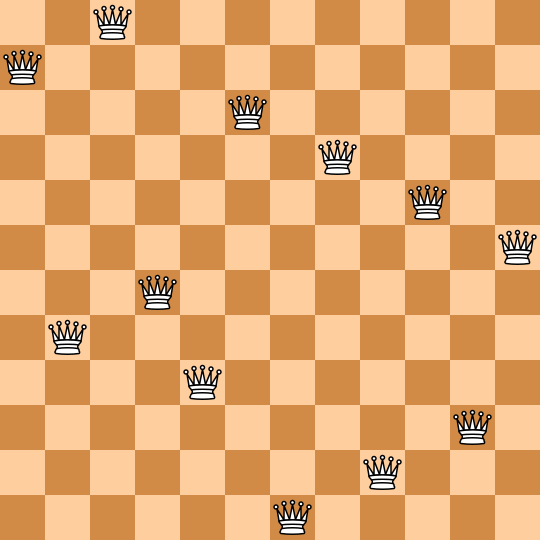
\includegraphics[scale=0.3]{board.png}
        \caption{Une solution au problème des $12$ dames}
        \end{figure}
	
	
\end{document}